\documentclass[conference]{IEEEtran}
\IEEEoverridecommandlockouts
% The preceding line is only needed to identify funding in the first footnote. If that is unneeded, please comment it out.
\usepackage{cite}
\usepackage{amsmath,amssymb,amsfonts}
\usepackage{algorithmic}
\usepackage{graphicx}
\usepackage{textcomp}
\usepackage{xcolor}
\def\BibTeX{{\rm B\kern-.05em{\sc i\kern-.025em b}\kern-.08em
    T\kern-.1667em\lower.7ex\hbox{E}\kern-.125emX}}
\begin{document}

\title{Autonomous Driving for the Texas Instruments Cup}

\author{\IEEEauthorblockN{Mohammed Fareed}
\IEEEauthorblockA{\textit{Kate Gleason College of Engineering} \\
\textit{Department of Computer Engineering}\\
Rochester, NY \\
mff9108@rit.edu}
\and
\IEEEauthorblockN{Trent Wesley}
\IEEEauthorblockA{\textit{Kate Gleason College of Engineering} \\
\textit{Department of Computer Engineering}\\
Rochester, NY \\
taw8452@rit.edu}
}

\maketitle

\begin{abstract}
	The field of autonomous driving promises enhanced road safety and efficiency. This paper details the implementation of an autonomous miniature car, designed to compete in the Rochester Institute of Technology's Texas Instruments Car Cup in Fall 2023. At the center of the car's control system is an MSP432 microcontroller, which processes data from a line-scan camera to dynamically adjust motor speed and steering servo for navigation. This project's core was the development and refinement of autonomous driving algorithms, addressing the intricate challenge of real-time sensor data processing and control. The results of this work is a demonstration of the car's capability to autonomously and independently navigate a racetrack, The experience provides insights into the practical application of theoretical concepts in autonomous systems.
\end{abstract}

\section{Introduction}
Each semester, the Rochester Institute of Technology (RIT) hosts the Texas Instruments (TI) autonomous car race, a practical challenge that encourages computer engineering students to apply their expertise in microcontrollers, motor control, control systems, and problem-solving to real-world scenarios. With the United States averaging 6 million car accidents annually, education and experience in autonomous driving can help shape a world where driving is much safer \cite{accidentStats}.

Participants in the TI Cup utilize custom-built cars comprising dual motors for rear-wheel drive, a servo for directional control, an MSP432 microcontroller board for central processing, a line-scan camera for path detection, an OLED display for diagnostics, and a 7.2V battery pack for power supply. Figure \ref{fig:car} illustrates the design of the competition vehicle.

\begin{figure}[htbp]
	\centerline{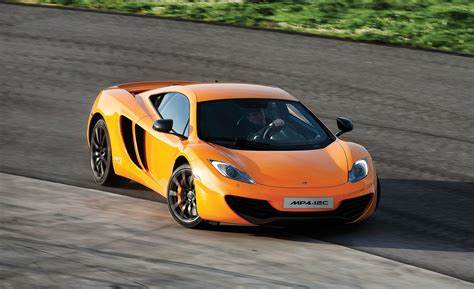
\includegraphics[width=0.45\textwidth]{images/car.jpg}}
	\caption{The autonomous car used in the TI Cup.}
	\label{fig:car}
\end{figure}

The competition track is designed to challenge the autonomous capabilities of the vehicles, featuring straightaways, turns, intersections, inclines, and undulating sections that test the precision and adaptability of the autonomous control systems.

The rest of this paper is organized as follows. Section 2 presents the background, including the TI Cup context, applied theories, MSP432 modules, and hardware components. Section 3 delineates the proposed methodologies and specific implementations. Section 4 discusses the race outcomes and the car's performance. Section 5 concludes the paper with reflections on the project's implications. Section 6 acknowledges contributions to the project, and Section 7 cites the references.

\section{Background}

\subsection{RIT TI Car Cup}

The RIT TI Car Cup is hosted every fall and spring semesters. In this event, teams are given three chances to set their fastest time for a single lap on a closed circuit. The clock stops the moment a team completes its first successful lap, which then becomes their official time record. If a team doesn't finish in three attempts, they are disqualified. For an lap to be considered successful, the car must finish in under 60 seconds and have at least two wheels on the track at all times. Race results were recorded by a laser timer for accuracy.

\subsection{Materials}

Constructing the autonomous car for the TI Cup required a diverse range of components. Referencing the specifications outlined in \cite{carCup2022}, a bill of materials was compiled, as detailed in Table \ref{table:billOfMaterials}.

\begin{table}[htbp]
\caption{Bill of Materials}
\begin{center}
\begin{tabular}{|c|c|c|}
\hline
Part & Qty & Cost (USD) \\
\hline
Parallax TSL-1401 Line Scan Camera & 1 & \$80.00 \\
\hline
Servo Steering Arms & 1 & \$17.99 \\
\hline
Motor Driver - RB-WAV-77 & 1 & \$28.9 \\
\hline
Car Chassis Kit - ROB0170 & 1 & \$98.75 \\
\hline
Brushed DC Motor Kit - KIT0167 & 1 & \$25.00 \\
\hline
UCTRONICS Module 12864 SSD1306 OLED & 1 & \$6.99 \\
\hline
Bluetooth Module HM-10 & 1 & \$10.99 \\
\hline
Tenergy 7.2V High Capacity 6-Cell Battery Pack & 1 & \$39.99 \\
\hline
Sourcingpower Universal RC Battery Charger & 1 & \$19.99 \\
\hline
Fielect 5Pcs F-F 6Pin Jumper Wire Ribbon Cable & 1 & \$6.69 \\
\hline
5pcs Tamiya Male Power Connector Cable & 1 & \$8.68 \\
\hline
Zip Ties & 1 & \$18.99 \\
\hline
\textbf{Total} & & \textbf{\$363.05} \\
\hline
\end{tabular}
\label{table:billOfMaterials}
\end{center}
\end{table}

The table shows each component's type, quantity, and cost in USD. The total cost to replicate the car with similar specifications is approximately \$363.05.

\subsection{Camera}

The autonomous vehicle utilized in the TI Cup features the Parallax TSL-1401 line-scan camera, a major component of the car's navigation system. This camera is designed to capture a one-dimensional array of light intensity across its field of view, using 128 photo-diodes arranged linearly. Each photo-diode corresponds to a pixel in the captured image, enabling the camera to detect variations in light intensity along a line.

The TSL-1401's capability to differentiate between light and dark areas is central to the car's ability to follow the track. In the context of the racetrack, which features distinct contrasts between the track (light) and the surroundings (dark), the camera provides real-time data for the microcontroller to process and determine the car's position relative to the track boundaries. This camera operates by scanning the track surface and generating an output signal that varies depending on the reflected light intensity. Brighter surfaces, like the white parts of the track, result in higher signal values, whereas darker areas, such as off-track surfaces or track borders, produce lower signal values. This difference in signal strength is what enables the autonomous vehicle to detect and stay within the track boundaries. Figure \ref{fig:camera} shows a wiring diagram for how the camera was connected to the MSP432.

\begin{figure}[htbp]
	\centerline{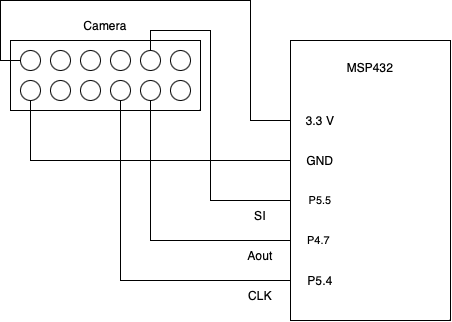
\includegraphics[width=0.45\textwidth]{images/cameraWiring.png}}
	\caption{Camera Wiring Diagram.}
	\label{fig:camera}
\end{figure}

The diagram shows that camera being powered by 3.3V and ground. The camera's SI, CLK, and AO pins are connected to P5.5, P4.7, and P5.4, respectively. The camera's AO pin is connected to the MSP432's ADC pin. The analog output from the camera is converted to a digital signal using the car's Analog to Digital Converter (ADC), allowing for precise digital processing and decision-making.

For optimal performance, the camera's placement angle and focus were carefully calibrated. The angle ensures that the camera has a clear and unobstructed view of the track ahead, while the focus is adjusted to maximize clarity and contrast in the captured image. This calibration was crucial in ensuring that the camera could reliably detect the contrast between the track and its surroundings under various lighting conditions encountered during the race.

\subsection{Motors}

The autonomous vehicle in the TI Cup was equipped with two key types of motors: Brushed DC Motor Kits (KIT0167) for propulsion and a servo motor for steering.

\textbf{Brushed DC Motors for Propulsion:} The rear wheels of the car were powered by two independently controlled Brushed DC Motors. Speed control was implemented through Pulse Width Modulation (PWM) signals, allowing for precise adjustments in motor speed in response to the track's demands.

\textbf{Servo Motor for Steering:} The car's steering mechanism was controlled by a servo motor. The servo's role was to precisely adjust the angle of the front wheels, enabling the car to follow the intended path on the racetrack. Implementing effective steering control was one of the project's significant challenges, requiring meticulous tuning to achieve optimal responsiveness and accuracy.

Figure \ref{fig:motorWiring} shows a wiring diagram for how the motors were connected to the MSP432.

\begin{figure}[htbp]
	\centerline{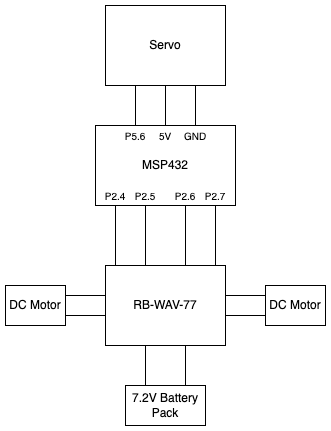
\includegraphics[width=0.45\textwidth]{images/motorsWiring.png}}
	\caption{Motor Wiring Diagram.}
	\label{fig:motorWiring}
\end{figure}

The diagram shows that the board had the motors interfaced using the RB-WAV-77 motor driver and the servo directly connected to the MSP432. motors were powered by 7.2V and ground, and their PWM pins were connected to P2.4-2.7, where each motor was assigned to a pair of pins. The direction of the DC motor was controlled by alternating the PWM signal between the two pins of the motor. The servo's PWM pin was connected to P5.6 and was powered by the on-board 5V and ground. Its angle was controlled by varying the PWM signal between 0.05 and 0.1 duty cycle.

\subsection{PID theory}

Proportional-Integral-Derivative (PID) control is a widely used feedback loop mechanism in control systems, including autonomous vehicles. This control strategy is crucial in maintaining a desired system behavior, such as steering and speed control in the context of autonomous racing. PID control is implemented by calculating an error value, which is the difference between the desired and actual system states. This error value is then used to adjust the system's behavior to minimize the error and achieve the desired state. The three components of PID control are as follows:

\begin{itemize}
	\item A PID controller continuously calculates an error value as the difference between a desired set point and a measured process variable. It then applies a correction based on proportional, integral, and derivative terms, denoted as P, I, and D, respectively.
	\item The \textbf{Proportional} term produces an output value proportional to the current error. In the autonomous vehicle, this helps to steer the car more aggressively when it deviates further from the track centerline.
	\item The \textbf{Integral} term focuses on the accumulation of past errors. It seeks to eliminate residual steady-state errors by integrating the error over time.
	\item The \textbf{Derivative} term predicts system behavior and thus can prevent the system from overshooting the setpoint. By reacting to the rate of change of the error, it provides a damping effect.
\end{itemize}

Figure \ref{fig:PID} shows a block diagram of a PID controller, illustrating how the feedback loop is implemented in the context of the car's steering and speed control systems.

\begin{figure}[htbp]
	\centerline{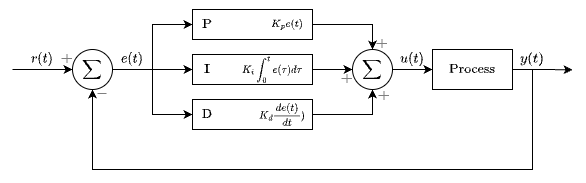
\includegraphics[width=0.45\textwidth]{images/pid.png}}
	\caption{PID Controller Block Diagram.}
	\label{fig:PID}
\end{figure}

The figure depicts the structured framework of the PID controller as implemented in our autonomous vehicle. The block diagram showcases three distinct paths representing the Proportional, Integral, and Derivative terms, each path applying a mathematical operation on the error signal $e(t)$. The Proportional path amplifies the error by a constant $K_p$, providing immediate correction proportional to the error. The Integral path integrates the error over time, scaled by $K_p$, to eliminate residual steady-state errors. The Derivative path, scaled by $k_d$, takes the derivative of the error, offering a predictive correction and dampening the system response to prevent overshoot.

These three signals converge at a summing junction, producing a combined output that dictates the control action to the process, which is the car's steering and throttle mechanism. This integration of responses ensures that the vehicle responds accurately to deviations from the desired trajectory, maintaining precise control throughout the race.

Tuning of the PID parameters ($K_p$, $K_i$, $K_d$) was a critical process in the solution design, involving iterative testing to achieve a balance between responsiveness and stability. The PID parameters were tuned to ensure that the car could follow the track's centerline while maintaining a reasonable speed. The PID controller was implemented in the car's code to control the steering servo, enabling the car to follow the track's centerline.

\subsection{Timers and Interrupts}

Effective timing and event management are critical in the control systems of autonomous vehicles. In our project, we utilized a suite of timers and interrupts on the MSP432 microcontroller to coordinate the activities of the motors, servo, and camera.

\textbf{Timer A0 for Motor PWM:} Timer A0 was dedicated to controlling the Pulse Width Modulation (PWM) for the Brushed DC Motors. By adjusting the timer period, the duty cycle of the PWM signal can be fine tuned, thus controlling the speed of the motors. This allowed for dynamic speed adjustments based on the car's immediate requirements for speed and precision on the track.

\textbf{Timer A2 for Servo PWM:} Similarly, Timer A2 was configured to manage the PWM for the servo motor responsible for steering. The precise timing of this timer was crucial for achieving smooth and responsive steering behavior, enabling the car to navigate the twists and turns of the racetrack with agility.

\textbf{Timer 32 and SysTick Timer for Camera Control:} The operation of the line-scan camera was managed by two timers. Timer 32 controlled the Start Integration (SI) signal, initiating the camera's capture sequence. In parallel, the SysTick Timer generated the clock (CLK) signal, ensuring that the camera's photo-diodes were sampled at consistent intervals for accurate light intensity readings.

\textbf{Interrupts:} Interrupts were used to manage the camera's output signal. The camera's analog output was connected to the MSP432's ADC pin, which was configured to trigger an interrupt when a new value was available. This interrupt sets a global boolean variable that is monitored by the main loop. The main loop would then read the camera's output and process the data to determine the car's position relative to the track boundaries.

\subsection{Analog to Digital Converter}

The Analog to Digital Converter (ADC) is a crucial component of the microcontroller that bridges the analog world with the digital system. In the autonomous vehicle, the ADC's primary role was to convert the analog signals from the Parallax TSL-1401 line-scan camera into digital values for processing and decision-making.

\textbf{Functionality of the ADC:}
\begin{itemize}
\item The TSL-1401 camera captures the track's image as an array of analog light intensities. The ADC on the MSP432 microcontroller translates these intensities into a series of digital values, which can range from 0 to $2^14 - 1$ (16383), representing a 14-bit resolution.
\item This high-resolution conversion is needed for distinguishing between the varying shades of gray that correspond to the track and its boundaries, allowing for finer control over the vehicle's steering and throttle based on the perceived path. Even slight variations in light intensity readings can lead to significant changes in the vehicle's trajectory. Thus, the accuracy of the ADC's conversions is vital.
\end{itemize}

\textbf{Integration with Control System:}
\begin{itemize}
\item Upon the ADC receiving analog values, the microcontroller's firmware is configured to initiate the ADC conversion process, which involves sampling the signal and converting it into a digital format.
\item The converted digital data is then fed into the PID control algorithms, informing the subsequent adjustments to the vehicle's motors and steering servo.
\item To ensure data accuracy and consistency, the ADC conversion process is synchronized with the camera's SI and CLK signals.
\end{itemize}

\section{Proposed Method}

\subsection{Camera Vision and Filtering}

The linescan camera's output is an array of 128 integers representing the brightness it sees. The linescan camera used had a maximum value of $2^{14}$-1 (16383), and would tend to saturate at that value pretty easily. This phenomenon was utilized to filter out the carpet from what was the track. If an array element was less than 16381, it wouldn't be considered as part of the track and would be treated as 0. Otherwise, the element would be treated as a 1. This creates a binary representation of track versus carpet. Figure \ref{fig:linescan} shows a plot characterizing the typical behavior of the linescan camera.

\begin{figure}[htbp]
	\centerline{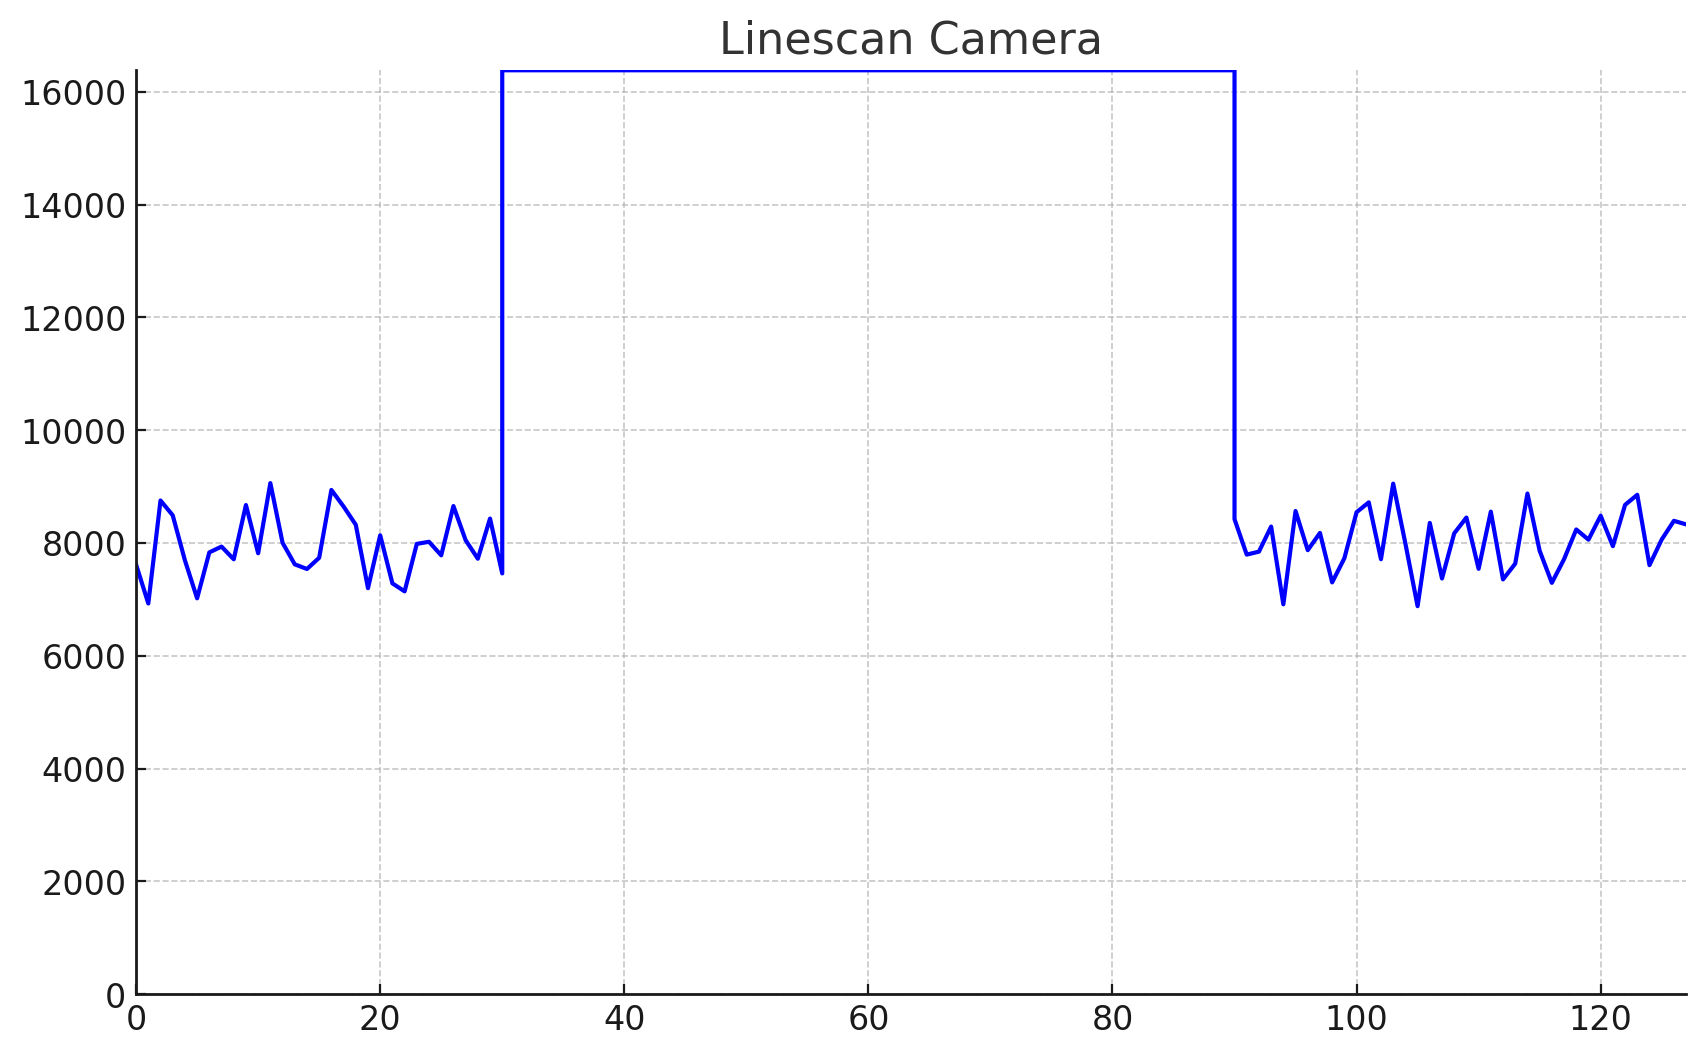
\includegraphics[width=0.45\textwidth]{images/linescan.png}}
	\caption{Unfiltered Linescan Output.}
	\label{fig:linescan}
\end{figure}

In Figure \ref{fig:linescan}, the saturated component is where the linescan camera sees the bright white track along the 128 elements of the array. The rest is the where the camera sees the darker carpet beside the track. As stated, this output was filtered into a binary representation of where there is and isn't track. This output is modeled by Figure \ref{fig:linescanFiltered}.

\begin{figure}[htbp]
	\centerline{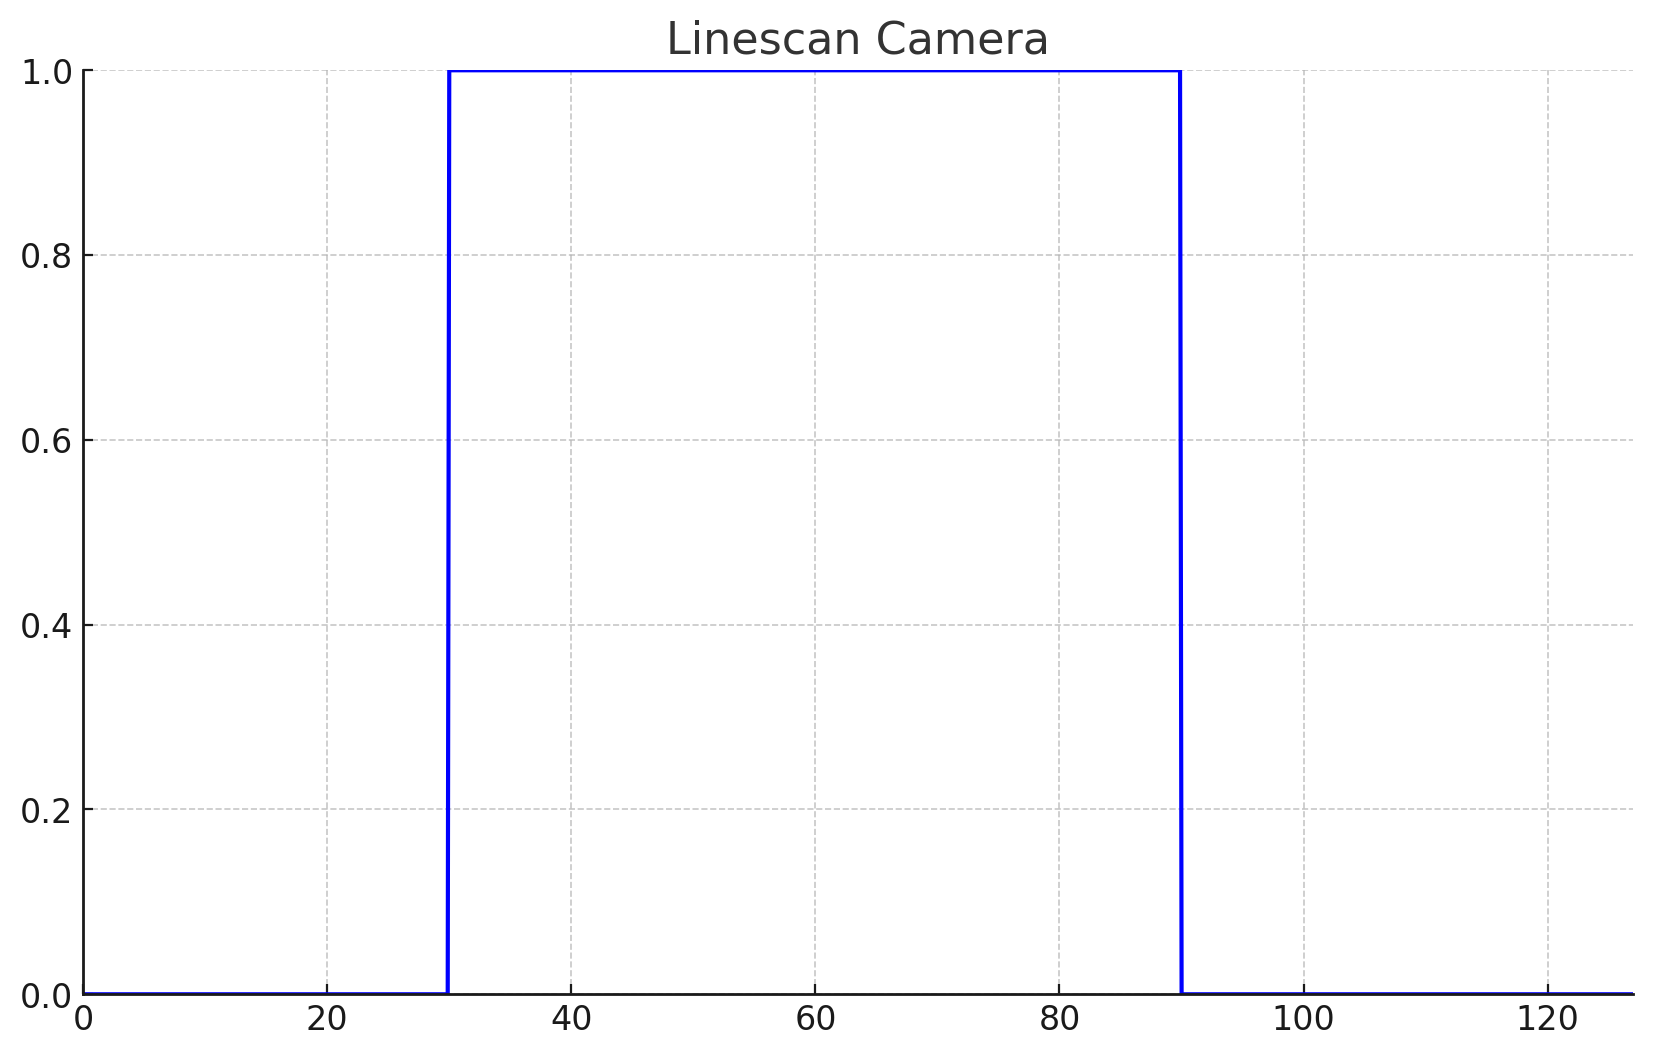
\includegraphics[width=0.45\textwidth]{images/linescanFiltered.png}}
	\caption{Filtered Linescan Output.}
	\label{fig:linescanFiltered}
\end{figure}

This filtered output is simpler and unbiased by the values unassociated with the track. Using the binary output, a weighted average was calculated to find where the center of the track is. The calculation is shown in Equation \ref{eq:midpoint}.

\begin{equation}
	\text{midpoint} = \frac{\sum_{i=0}^{127} i*x_i}{\sum_{i=0}^{127} x_i}\label{eq:midpoint}
\end{equation}

In Equation \ref{eq:midpoint}, $i$ represents the index in the array and $x_i$ represents the binary value at the index in the array. The resulting midpoint can the be used to determine the position of the middle of the track and steer towards it.

This binary representation simplifies the process of distinguishing track boundaries, enabling more accurate steering control as the car navigates the varying contrasts of the racetrack.

\subsection{Carpet Detection}

Carpet detection is important for preventing damage from hitting a wall when the car would drive off the track. The program logic created to detect whether the car has left the track is very simple. Every element of the raw output array from the linescan camera was added up. This sum was compared to a brightness threshold calibrated through trial and error. If the sum was less that the threshold, the car would stop the DC motors and therefore stop the car from moving.

This feature plays a major role in preventing potential damage to the vehicle, especially in scenarios where the car veers off-track or bumps into other cars, ensuring the safety and longevity of the equipment during testing.

\subsection{PID Implementation}


The Proportional-Integral-Derivative (PID) control system was utilized for steering with a servo to be able to handle turns and reduce oscillations on straight paths. Error is an essential variable for PID to function. For this project, error was the calculated as shown in Equation \ref{eq:error}.

\begin{equation}
	\text{error} = \text{midpoint} - 64.5 \label{eq:error}
\end{equation}

On a scale from 0 to 127 (indices of linescan camera output), the midpoint would normally be 63.5. In this case, it was 64.5 to adjust for the offset of the camera. This calculated error was then utilized for the PID control of the servo. The formula for the PID control system is shown in Equation \ref{eq:PID}.

\begin{equation}
	\begin{aligned}
		\text{ServoPWM} &= K_p \times \text{error1} \\
					&+ K_i \times \left( \frac{\text{error1} + \text{error2} + \text{error3}}{3} \right) \\
					&+ K_d \times (\text{error1} - 2 \times \text{error2} + \text{error3})
	\end{aligned}
	\label{eq:PID}
\end{equation}

In Equation 3:
\begin{itemize}
\item \text{error1} represents the most recent error measurement.
\item \text{error2} is the error measurement preceding \text{error1}.
\item \text{error3} denotes the error measurement before \text{error2}.
\end{itemize}
This approach of incorporating a history of error measurements enables the PID algorithm to optimize the vehicle's response, not just based on the most recent error but by considering its previous states as well.

This calculation alone is not sufficient since a servo PWM outside of the range 0.05 to 0.1 could break the car. For this reason, code was added which would set the servo's PWM to 0.05 if the calculated value was less than 0.05. Additionally, the code would set the servo's PWM to 0.1 if the calculated value was greater than 0.1.

\subsection{Variable Speed}

Variable speed was implemented so that the car would slow down when turning and speed up when going straight. Specifically, this was implemented with an equation relating the absolute value of servo's PWM input (0.05 to 0.1 duty cycle) minus its middle position (0.075 duty cycle). The more the servo position varied from the center, the slower the car was programmed to go. This is shown in Equation \ref{eq:speed}.

\begin{equation}
	\text{MotorPWM} = -18*|\text{ServoPWM} - 0.075| + 0.434 \label{eq:speed}
\end{equation}

If the motor PWM calculated is less than 0.36, it was set to 0.36 by the code to ensure it was maintaining a decently fast speed.

Implementing variable speed control allowed the car to change its speed dynamically, slowing down for sharp turns and accelerating on straight segments. This was essential for optimizing the car's speed across the track, minimizing the time required to complete a lap.

\section{Results}

\subsection{Race Results}

The Texas Instruments Cup race was held on December 2nd, 2023. The track layout for the race is depicted in Figure \ref{fig:track}.

\begin{figure}[htbp]
	\centerline{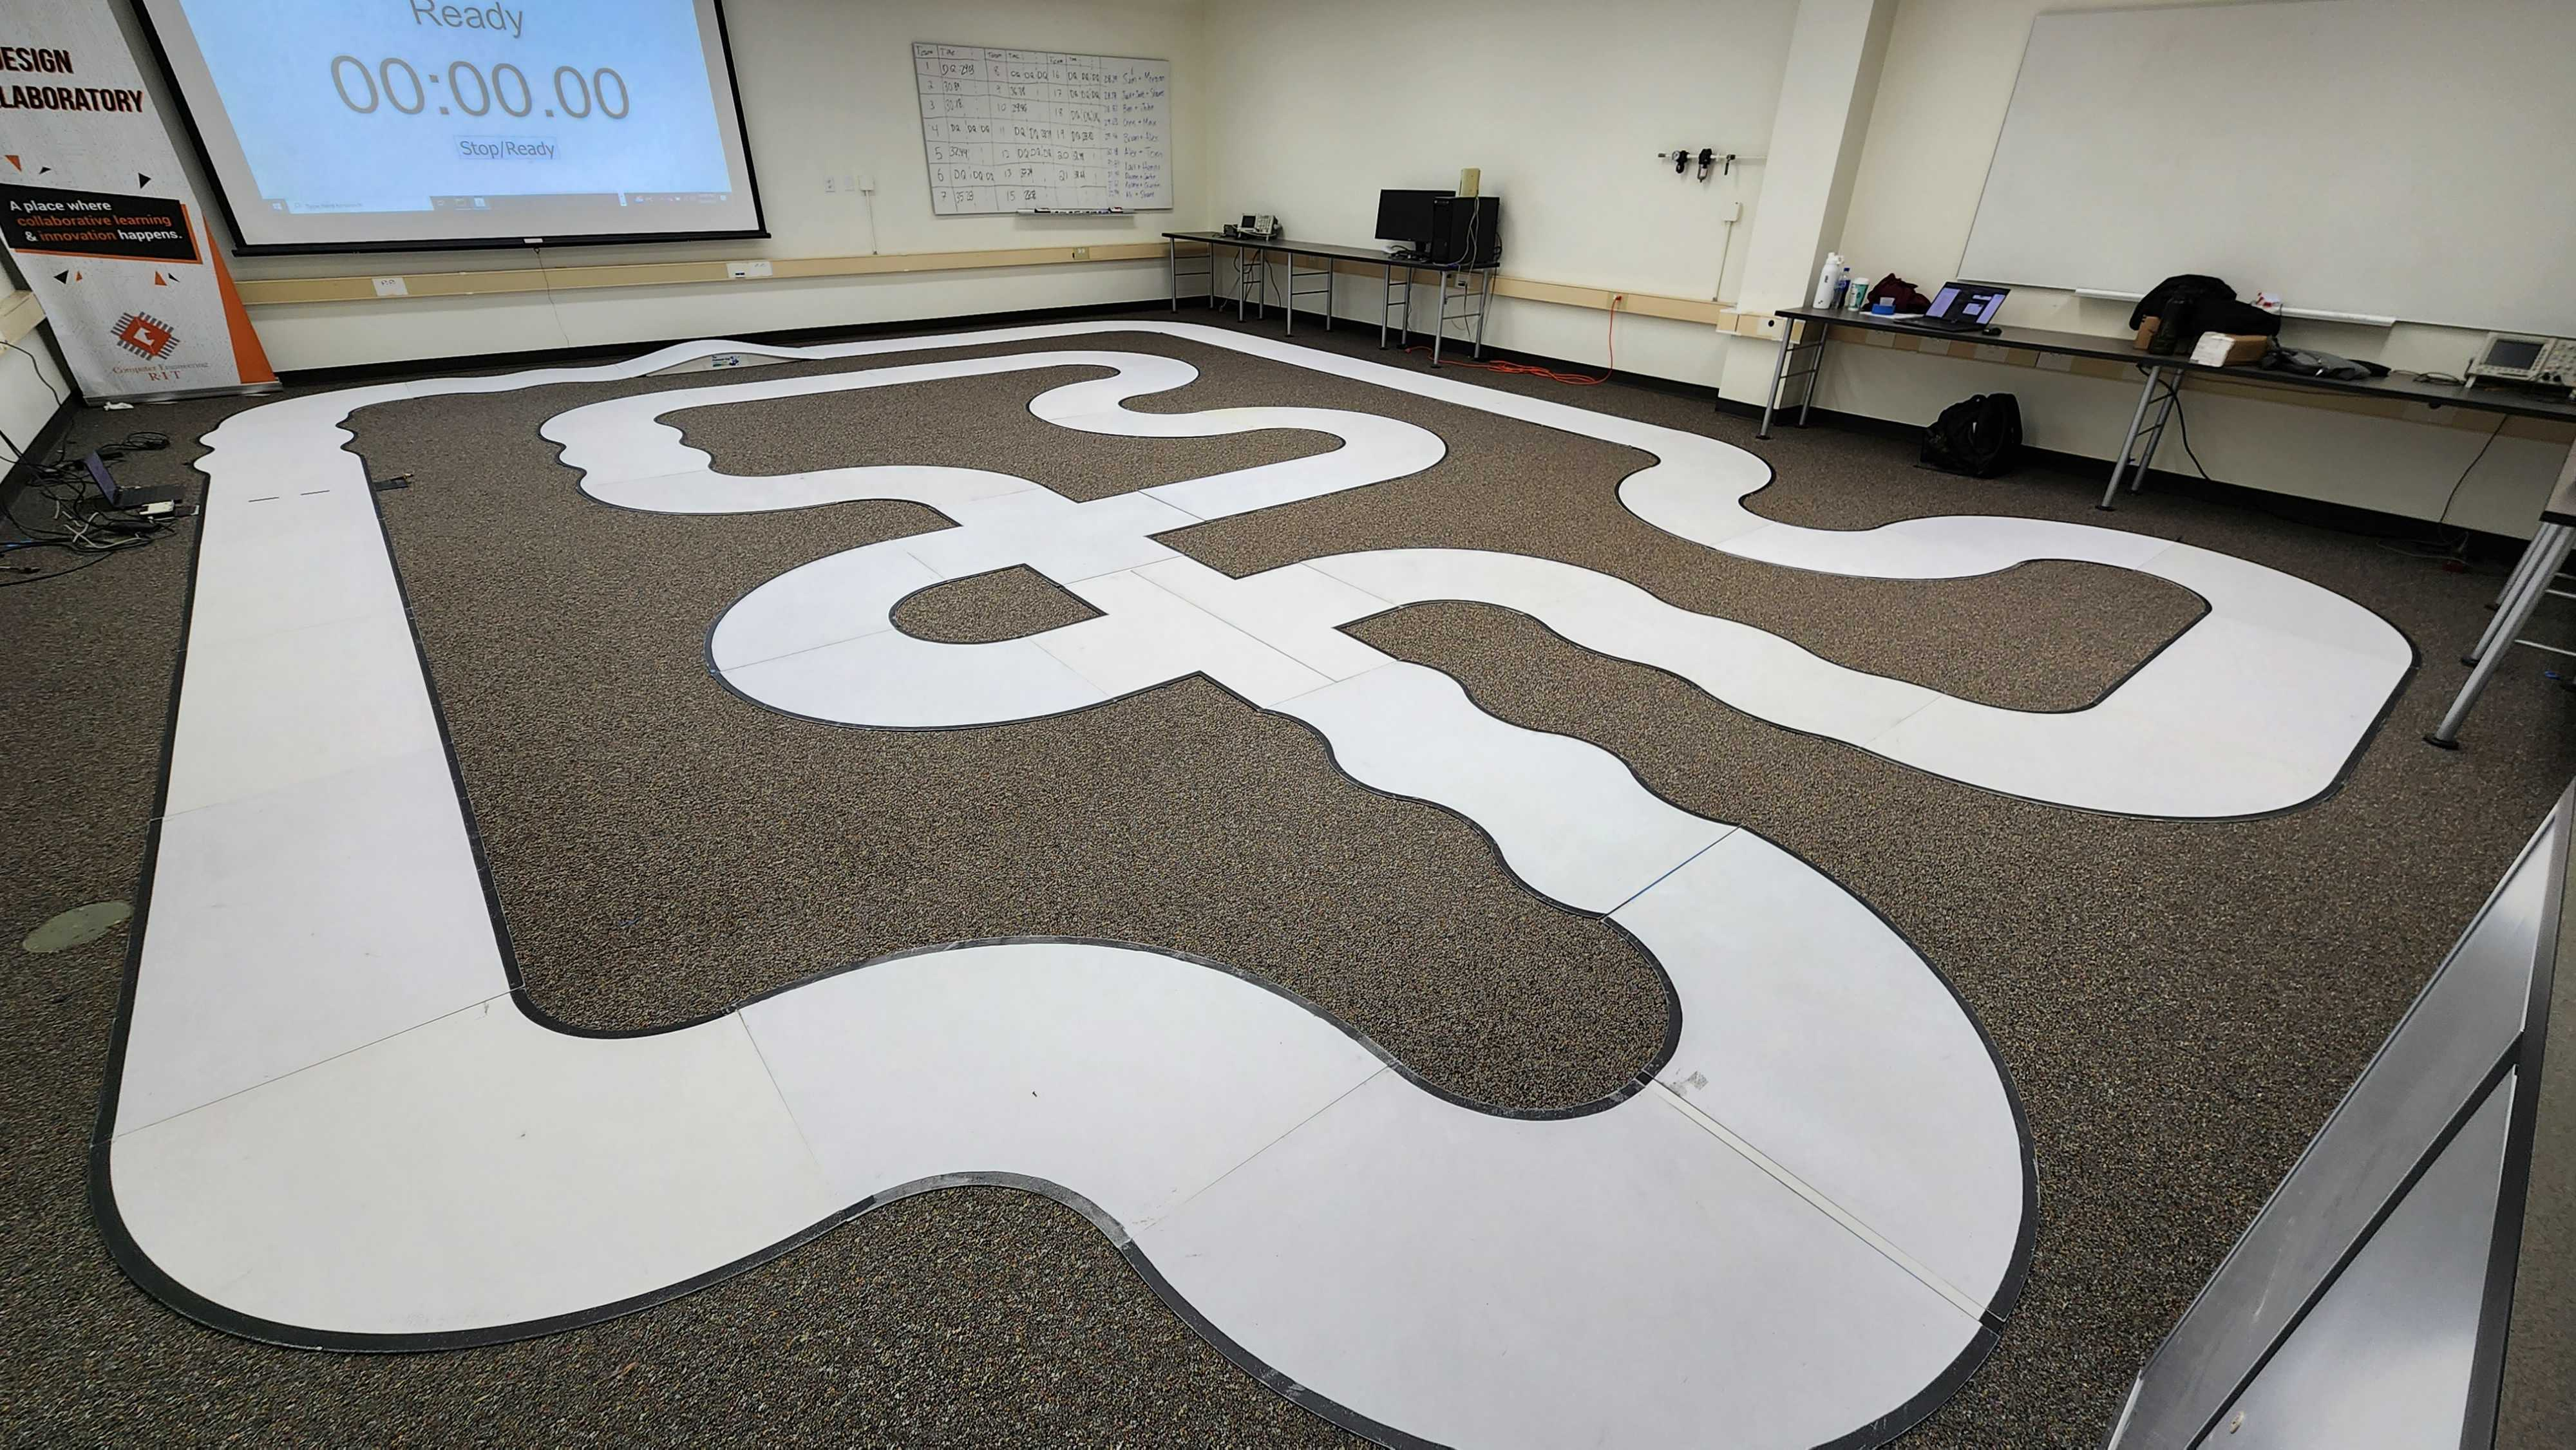
\includegraphics[width=0.45\textwidth]{images/track.jpg}}
	\caption{Racetrack for TI Cup.}
	\label{fig:track}
\end{figure}

The final track design, featuring a crossed-U shaped section with squiggly paths following a ramp, presented a unique challenge that tested the limits of the car's capabilities. In the practice run, the car showcased promising performance, with minor issues. Notably, the car struggled with speed control after the ramp and exhibited oscillatory behavior on straight sections, veering left and right.

On race day, each team had three attempts to complete the track with the fastest possible time. the authors' team, team number four, approached the race with a single driving mode that they believed to be the best after PID tuning. Although experiments with differential driving were performed as a potential second mode, it was not deployed due to insufficient testing to ensure its reliability during the race.

The car's performance in the actual race, unfortunately, did not reflect the success of the practice rounds. During our attempts, the line-scan camera experienced a failure, which compromised the vehicle's ability to detect the track correctly. This technical issue led to our car being unable to complete the track, marking a disqualification (DQ) in the final results as shown in Table \ref{tab:raceResults}.

\begin{table}[htbp]
	\caption{Race Day Results}
	\begin{center}
	\begin{tabular}{|c|c|c|c|c|}
		\hline
		\textbf{Team} & \textbf{Attempt 1} & \textbf{Attempt 2} & \textbf{Attempt 3} & \textbf{Final Time (s)} \\
		\hline
		1 & Q & 29.03 & - & 29.03 \\
		2 & 30.84 & - & - & 30.84 \\
		3 & 30.18 & - & - & 30.18 \\
		\textbf{4} & \textbf{DQ} & \textbf{DQ} & \textbf{DQ} & \textbf{DQ} \\
		5 & 32.44 & - & - & 32.44 \\
		6 & DQ & DQ & DQ & DQ \\
		7 & 35.28 & - & - & 35.28 \\
		8 & DQ & DQ & DQ & DQ \\
		9 & 36.39 & - & - & 36.39 \\
		10 & 29.46 & - & - & 29.46 \\
		11 & DQ & DQ & 29.39 & 29.39 \\
		12 & DQ & DQ & DQ & DQ \\
		13 & 37.24 & - & - & 37.24 \\
		14 & 28.58 & - & - & 28.58 \\
		15 & 28.82 & - & - & 28.82 \\
		16 & DQ & DQ & DQ & DQ \\
		17 & DQ & DQ & DQ & DQ \\
		18 & DQ & DQ & DQ & DQ \\
		19 & DQ & 28.82 & - & 28.82 \\
		20 & 31.49 & - & - & 31.49 \\
		21 & 31.61 & - & - & 31.61 \\

		\hline
	\end{tabular}
	\label{tab:raceResults}
	\end{center}
\end{table}

The race results show that the top three teams were able to complete the track in under 29 seconds, with the fastest time being 28.39 seconds. Most teams that did not get disqualified for not completing the race locked-in their time on the first attempt, with only 2 teams in the second and a single in the third. In total, 7 teams out of 21 were disqualified for not completing the track, including the authors' team.

Despite the setback, the data obtained from the practice run and partial race attempts have provided valuable insights. The race results of the car, while not resulting in a completed lap, reflects the challenges of real-world autonomous vehicle applications.

\section{Conclusion}

The TI Car Cup competition is an example of how to turn a real-world engineering problem into an engaging course activity. With autonomous cars becoming more prevalent, this provides a good opportunity for students to get hands-on experience with what goes into making these types of vehicles function. This project serves as a capstone project for the Interfaces and Digital Electronics class, requiring students to incorporate everything they have learned throughout the semester to be successful. This includes not only technical skills like programming and understanding electronics but also soft skills like project management, time management, and teamwork. Using all these skills, a solution was implemented that was able to successfully navigate the track in practice runs. Although the car was unable to complete the track during the race, the performance of competing cars provided valuable lessons. The results showed the competitive nature of the challenge and the narrow margins that separate the top contenders. Future iterations of the project could benefit from further tuning of the PID algorithm and control loop for even more efficient steering and acceleration. Further testing of the differential driving mode could also be performed to determine its viability as a second driving mode.

\section{Acknowledgments}

The authors would like to thank Dr. Hussin Ketout for his guidance throughout the Texas Instruments Cup project. His expertise in autonomous systems was invaluable. Appreciation is also extended to teaching assistants Andrew Tevebaugh, Colin Vo, and Ben Hyman for their technical support and assistance during the project's development phase. Their contributions to the troubleshooting process significantly enhanced the project's outcome.

\begin{thebibliography}{00}
\bibitem{accidentStats} “Car Accident Statistics in the U.S. | Driver Knowledge,” DriverKnowledge, 2019. https://www.driverknowledge.com/car-accident-statistics/
\bibitem{carCup2022} K. Jacowleff and M. Teichman, “Texas Instruments Autonomous Car Cup Project Fall 2022,” 2022.
\end{thebibliography}
\end{document}
